\chapter{ĐẶC TẢ YÊU CẦU PHẦN MỀM}

\section{Tổng quan sản phẩm}

\subsection{Mô tả hệ thống}

SmartDroneDelivery là nền tảng quản lý giao hàng bằng drone tích hợp AI, được xây dựng để hỗ trợ doanh nghiệp quản lý toàn bộ quy trình giao hàng. Hệ thống cho phép quản lý khách hàng, đơn giao hàng, kiện hàng, drone và trạm hạ cánh, đồng thời hỗ trợ điều phối, theo dõi và xác nhận giao hàng.

Hệ thống tích hợp AI để dự đoán thời gian giao hàng (ETA), tóm tắt quá trình giao hàng, hỗ trợ khách hàng và phân tích dữ liệu vận hành. Nền tảng được cung cấp qua Web Application, Mobile Application và RESTful API, giúp các bên liên quan quản lý và theo dõi hoạt động giao hàng hiệu quả.

\subsection{Sơ đồ ngữ cảnh}

\begin{figure}[H]
\centering
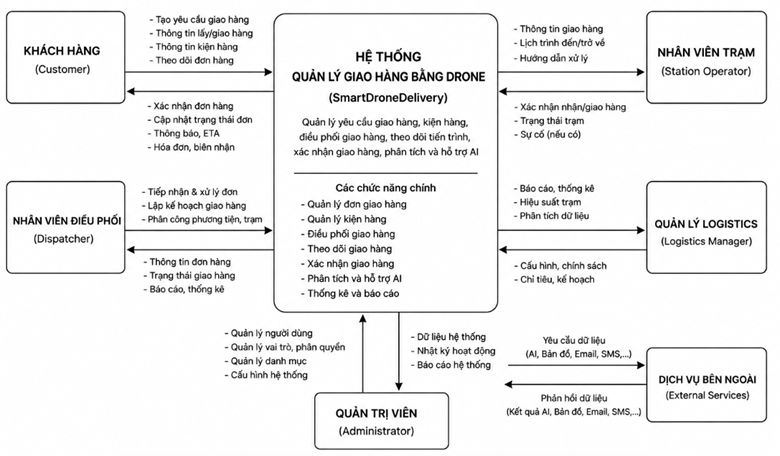
\includegraphics[width=6.5in,height=3.80278in,keepaspectratio,width=\linewidth]{images/Sơ đồ ngữ cảnh.png}
\end{figure}

\subsection{Quy trình nghiệp vụ chính}

Quy trình bắt đầu khi Khách hàng tạo yêu cầu giao hàng và kết thúc khi đơn hàng được giao thành công hoặc được xác định là giao thất bại.

\begin{enumerate}
\def\labelenumi{\arabic{enumi}.}
\item
  Tạo yêu cầu giao hàng: Khách hàng nhập thông tin người nhận, địa chỉ và kiện hàng, sau đó gửi yêu cầu.
\item
  Tiếp nhận và duyệt đơn: Nhân viên điều phối kiểm tra thông tin và phê duyệt hoặc từ chối yêu cầu.
\item
  Lập kế hoạch giao hàng: Hệ thống hỗ trợ xác định thời gian giao, drone và trạm hạ cánh phù hợp.
\item
  Tiếp nhận kiện hàng: Nhân viên trạm kiểm tra và xác nhận kiện hàng.
\item
  Thực hiện giao hàng: Drone vận chuyển kiện hàng theo kế hoạch.
\item
  Theo dõi giao hàng: Hệ thống cập nhật trạng thái, tiến độ và ETA để khách hàng và nhân viên theo dõi.
\item
  Xác nhận kết quả: Người nhận xác nhận đã nhận hàng. Nếu giao thất bại, nhân viên điều phối xử lý giao lại hoặc hủy đơn.
\end{enumerate}

